% ****** Start of file apssamp.tex ******
%
%   This file is part of the APS files in the REVTeX 4.2 distribution.
%   Version 4.2a of REVTeX, December 2014
%
%   Copyright (c) 2014 The American Physical Society.
%
%   See the REVTeX 4 README file for restrictions and more information.
%
% TeX'ing this file requires that you have AMS-LaTeX 2.0 installed
% as well as the rest of the prerequisites for REVTeX 4.2
%
% See the REVTeX 4 README file
% It also requires running BibTeX. The commands are as follows:
%
%  1)  latex apssamp.tex
%  2)  bibtex apssamp
%  3)  latex apssamp.tex
%  4)  latex apssamp.tex
%
\documentclass[%
 reprint,prl, %% for final paper
superscriptaddress,
%groupedaddress,
%unsortedaddress,
%runinaddress,
%frontmatterverbose, 
%preprint, %% for single-column, double-spacing
%preprintnumbers,
%nofootinbib,
nobibnotes,
%bibnotes,
 amsmath,amssymb,
 aps,
%pra,
%prb,
%rmp,
%prstab,
%prstper,
%floatfix,
]{revtex4-2}
\usepackage[utf8]{inputenc}
\usepackage{graphicx}% Include figure files
\usepackage{dcolumn}% Align table columns on decimal point
\usepackage{bm}% bold math
\usepackage{hyperref}% add hypertext capabilities
\usepackage[mathlines]{lineno}% Enable numbering of text and display math
\usepackage{amsmath} %for multiline in equation
%\usepackage{comment}

%\linenumbers %for preprint
\relax % Commence numbering lines
%\usepackage[showframe,%Uncomment any one of the following lines to test 
%%scale=0.7, marginratio={1:1, 2:3}, ignoreall,% default settings
%%text={7in,10in},centering,
%%margin=1.5in,
%%total={6.5in,8.75in}, top=1.2in, left=0.9in, includefoot,
%%height=10in,a5paper,hmargin={3cm,0.8in},
%]{geometry}

%abbreviation
\newcommand{\gagg}{\ensuremath{\left|g_{a\gamma\gamma}\right|}}
\newcommand{\ggamma}{\ensuremath{\left|g_{\gamma}\right|}}
\newcommand{\bgagg}{\ensuremath{g_{a\gamma\gamma}}}
\newcommand{\bggamma}{\ensuremath{g_{\gamma}}}
\newcommand{\ma}{\ensuremath{m_a}}
\newcommand{\tsys}{\ensuremath{T_\text{sys}}}
\newcommand{\ta}{\ensuremath{T_\text{a}}}
\newcommand{\muevcc}{\ensuremath{\,\mu\text{e\hspace{-.08em}V}}}
\newcommand{\MeV}{\ensuremath{\,\text{Me\hspace{-.08em}V}}}
\newcommand{\GeV}{\ensuremath{\,\text{Ge\hspace{-.08em}V}}}
\newcommand{\GeVinv}{\ensuremath{\,\text{Ge\hspace{-.08em}V}^{-1}}}
\newcommand{\flo}{\ensuremath{4.70750}}
\newcommand{\fhi}{\ensuremath{4.79815}}
\newcommand{\mlo}{\ensuremath{19.4687}}
\newcommand{\mhi}{\ensuremath{19.8436}}
\newcommand{\avelimit}{\ensuremath{8.2\times 10^{-14}}} %8.19+-0.38       
\newcommand{\ADMXavelimit}{\ensuremath{4.9\times 10^{-14}}}
\newcommand{\lolimit}{\ensuremath{5.3\times 10^{-14}}}
\newcommand{\hilimit}{\ensuremath{8.9\times 10^{-14}}}
\newcommand{\noise}{\ensuremath{1.9 - 2.2}}




\begin{document}

\preprint{APS/123-QED}

%\title{First Results from the Taiwan Axion Search Experiment with Haloscope in the \mlo--\mhi\muevcc\ Mass Range}% Force line breaks with \\
\title{First Results from the Taiwan Axion Search Experiment with Haloscope at 19.6\muevcc}% Force line breaks with \\

%Hsin Chang
\author{Hsin~Chang}\affiliation{Department of Physics, National Central University, Taoyuan City 320317, Taiwan}
%Jing-Yang Chang
\author{Jing-Yang~Chang}\affiliation{Department of Physics, National Central University, Taoyuan City 320317, Taiwan} 
%Yi-Chieh Chang
\author{Yi-Chieh~Chang}\affiliation{National Synchrotron Radiation Research Center, Hsinchu 300092, Taiwan} 
%Yu-Han Chang
\author{Yu-Han~Chang}\affiliation{Department of Physics, National Chung Hsing University, Taichung City 402202, Taiwan}
%Yuan-Hann Chang
\author{Yuan-Hann~Chang}\affiliation{Institute of Physics, Academia Sinica, Taipei City 115201, Taiwan}
\affiliation{Center for High Energy and High Field Physics, National Central University, Taoyuan City 320317, Taiwan}
%Chien-Han CHen
\author{Chien-Han~Chen}\affiliation{Institute of Physics, Academia Sinica, Taipei City 115201, Taiwan} 
%Ching-Fang Chen 
\author{Ching-Fang~Chen}\affiliation{Department of Physics, National Central University, Taoyuan City 320317, Taiwan}
%Kuan-Yu CHen
\author{Kuan-Yu~Chen}\affiliation{Department of Physics, National Central University, Taoyuan City 320317, Taiwan} 
%Yung-Fu Chen
\author{Yung-Fu~Chen}\email[Correspondence to: ]{yfuchen@ncu.edu.tw}\affiliation{Department of Physics, National Central University, Taoyuan City 320317, Taiwan} 
%Wei-Yuan James Chiang
\author{Wei-Yuan~Chiang}\affiliation{National Synchrotron Radiation Research Center, Hsinchu 300092, Taiwan}
%Wei-Chen Chien
\author{Wei-Chen~Chien}\affiliation{Department of Physics, National Chung Hsing University, Taichung City 402202, Taiwan}
%Hien Thi Doan
\author{Hien~Thi~Doan}\affiliation{Institute of Physics, Academia Sinica, Taipei City 115201, Taiwan} 
%Wei-Cheng Hung
\author{Wei-Cheng~Hung}\affiliation{Department of Physics, National Central University, Taoyuan City 320317, Taiwan}\affiliation{Institute of Physics, Academia Sinica, Taipei City 115201, Taiwan} 
%Watson Kuo
\author{Watson~Kuo}\affiliation{Department of Physics, National Chung Hsing University, Taichung City 402202, Taiwan} 
%Shou-Bai Lai
\author{Shou-Bai~Lai}\affiliation{Department of Physics, National Central University, Taoyuan City 320317, Taiwan} 
%Han-Wen Liu
\author{Han-Wen~Liu}\affiliation{Department of Physics, National Central University, Taoyuan City 320317, Taiwan} 
%Min-Wei Ouyang
\author{Min-Wei~OuYang}\affiliation{Department of Physics, National Central University, Taoyuan City 320317, Taiwan}
%Ping-I Wu
\author{Ping-I~Wu}\affiliation{Department of Physics, National Central University, Taoyuan City 320317, Taiwan} 
%Shin-Shan Yu
\author{Shin-Shan~Yu}\email[Correspondence to: ]{syu@phy.ncu.edu.tw}\affiliation{Department of Physics, National Central University, Taoyuan City 320317, Taiwan}
\affiliation{Center for High Energy and High Field Physics, National Central University, Taoyuan City 320317, Taiwan}


\collaboration{TASEH Collaboration}%\noaffiliation




\date{\today}% It is always \today, today,
             %  but any date may be explicitly specified

\begin{abstract}

 This Letter reports on the first results from the 
Taiwan Axion Search Experiment with Haloscope, a search for axions 
using a microwave cavity at frequencies between \flo\ and \fhi~GHz. 
Apart from the non-axion signals, no candidates with 
a significance more than 3.355 were found. The experiment excludes 
models with the axion-two-photon coupling $\gagg\gtrsim \avelimit\GeVinv$, 
a factor of eleven above the benchmark 
KSVZ model, reaching 
a sensitivity three orders of magnitude better than any existing limits 
 in the mass range $\mlo < \ma < \mhi \muevcc$.  
 It is also the first time that a haloscope-type experiment places 
constraints on the \bgagg\ in this mass region.


%\begin{description}
%\item[Usage]
%Secondary publications and information retrieval purposes.
%\item[Structure]
%You may use the \texttt{description} environment to structure your abstract;
%use the optional argument of the \verb+\item+ command to give the category of each item. 
%\end{description}
\end{abstract}

%\keywords{Suggested keywords}%Use showkeys class option if keyword
                              %display desired
\maketitle

%\tableofcontents %for preprint
%%%%%%%%%%%%%%%%%%%%%%%%%%%%%%%%%%%%%%%%%%%%%%%%%%%%%%%%%%%%%%%%%%%%%%%%%%%%%%%
%%% Introduction} 
Various astrophysical and cosmological observations indicate that dark matter 
(DM) exists and makes up 26.4\% of the total energy density of the 
universe~\cite{DMI,DMII,DMIII,DMIV,PDG}. One of the viable dark matter 
candidates is the axion, which arises from the spontaneous breaking of a new 
global U(1)$_\mathrm{PQ}$ symmetry~\cite{strongCPI}  
introduced by Peccei and Quinn to solve the strong CP 
problem~\cite{strongCPI,strongCPII,strongCPIII}. 
Axions are abundantly produced during the QCD phase transition in 
the early universe and may constitute the 
DM~\cite{ADDONI,ADDONII,ADDONIII,ADDONIV}. 
In the post-inflationary PQ symmetry breaking scenario, 
%where the PQ symmetry is broken after inflation, 
current calculations suggest a mass range of 
${\cal O}(1–100)$~\muevcc\ for axions so that the cosmic axion density does 
not exceed the 
observed cold DM density~\cite{QCDCalI,QCDCalII,QCDCalIII,QCDCalIV,QCDCalV,QCDCalVI,QCDCalVII,QCDCalVIII,QCDCalIX,QCDCalX,QCDCalXI,QCDCalXII,QCDCalXIII}. 
%Therefore, axions are compelling because they may explain at the same 
%time two puzzles that are on scales different by more than thirty orders of 
%magnitude. 
%

Axions could be detected and studied via their two-photon interaction, 
%the so-called ``inverse Primakoff effect'', 
of which the strength is described by the coupling constant \bgagg. 
The detectors with the best sensitivities to axion DMs with a mass of 
$\ma\approx \muevcc$, as first proposed by 
Sikivie~\cite{SikivieI,SikivieII}, are haloscopes consisting of a microwave 
(MW) cavity immersed in a strong static 
magnetic field and operated at a cryogenic temperature. 
In the presence of an external magnetic field, the ambient oscillating axion 
field drives the cavity and they resonate when the frequencies of the 
electromagnetic 
modes in the cavity match the MW frequency $f$, where $f$ is set by 
the total energy of the axion: $hf=E_a=\ma c^2 + \frac{1}{2}\ma v^2$. The 
axion signal power is further delivered 
to the readout probe followed by a low-noise linear amplifier. 
%The axion mass is unknown, therefore, 
%the cavity resonator must allow the possibility to be tuned through a range
%of possible axion masses. 

Several haloscope experiments have actively carried out axion searches. 
The most significant efforts are from the Axion Dark Matter 
eXperiment (ADMX), placing tight constraints on the \bgagg\ 
within the mass range of 
1.9--4.2\muevcc~\cite{ADMXI,ADMXII,ADMXIII,ADMXIV,ADMXV,ADMXVI,ADMXVII}. 
Others include the Haloscope at Yale Sensitive to Axion Cold dark matter 
(HAYSTAC)~\cite{HAYSTACIII,HAYSTACIV,HAYSTACI}, the Center 
for Axion and Precision Physics Research (CAPP)~\cite{CAPPII,CAPPIII,CAPPI}, 
and the QUest for AXions-$a\gamma$ (QUAX-$a\gamma$)~\cite{QUAX}. 
%
This Letter presents the first results 
of a search for axions in the mass range of \mlo--\mhi\muevcc, 
from the Taiwan Axion Search Experiment with Haloscope (TASEH). 

%% Experimental Setup 
The detector of TASEH is located at the Department of Physics, National 
Central University, Taiwan and housed within a cryogen-free 
dilution refrigerator (DR) from BlueFors. An 8-Tesla 
superconducting solenoid with a 
bore diameter of 76~mm and a length of 240 mm is integrated with the DR.  
The DR has multiple flanges at different temperatures for 
the required cooling: 50K, 4K, still, 
and mixing flanges, among which the mixing flange could reach the lowest 
temperature at $\simeq20$~mK. 
%
During the data taking, the MW cavity with two coupling probes 
sits in the center of the magnet bore 
and is connected via holders to the mixing flange. 
The $0.234$-L cylindrical cavity, 
made of oxygen-free high-conductivity (OFHC) copper, 
has an inner radius of 2.5~cm and a height of 12~cm and 
 is split into two halves along the axial direction to reduce the loss from 
the seam~\cite{CAPPCavity}. 
The resonant frequency can be tuned via the rotation of an off-axis OFHC 
copper tuning rod. 
The axion-photon conversion signal from the readout probe is directed to an 
impedance-matched amplification chain (thick lines in Fig.~\ref{fig:TASEH}). 
The first-stage amplifier is a low noise high-electron-mobility-transistor 
(HEMT) amplifier mounted on the 4K flange. 
A circulator, anchored at the mixing flange, 
prevents thermal radiation from the HEMT amplifier back 
streaming to the cold cavity and then being reflected.  
The signal is further amplified at room temperature via a 
three-stage post-amplifier, and down-converted 
and demodulated to in-phase (I) and quadrature (Q) components and digitized 
by an analog-to-digital converter with a sampling rate of 2~MHz. 
Two heavily attenuated input 
lines support scattering parameter measurements of the cavity and transmit 
test signals. 
Figure~\ref{fig:TASEH} shows a simplified diagram of the TASEH apparatus. 
More details of the TASEH detector can be found 
in Ref.~\cite{TASEHInstrumentation}. 

\begin{figure} 
  \centering
  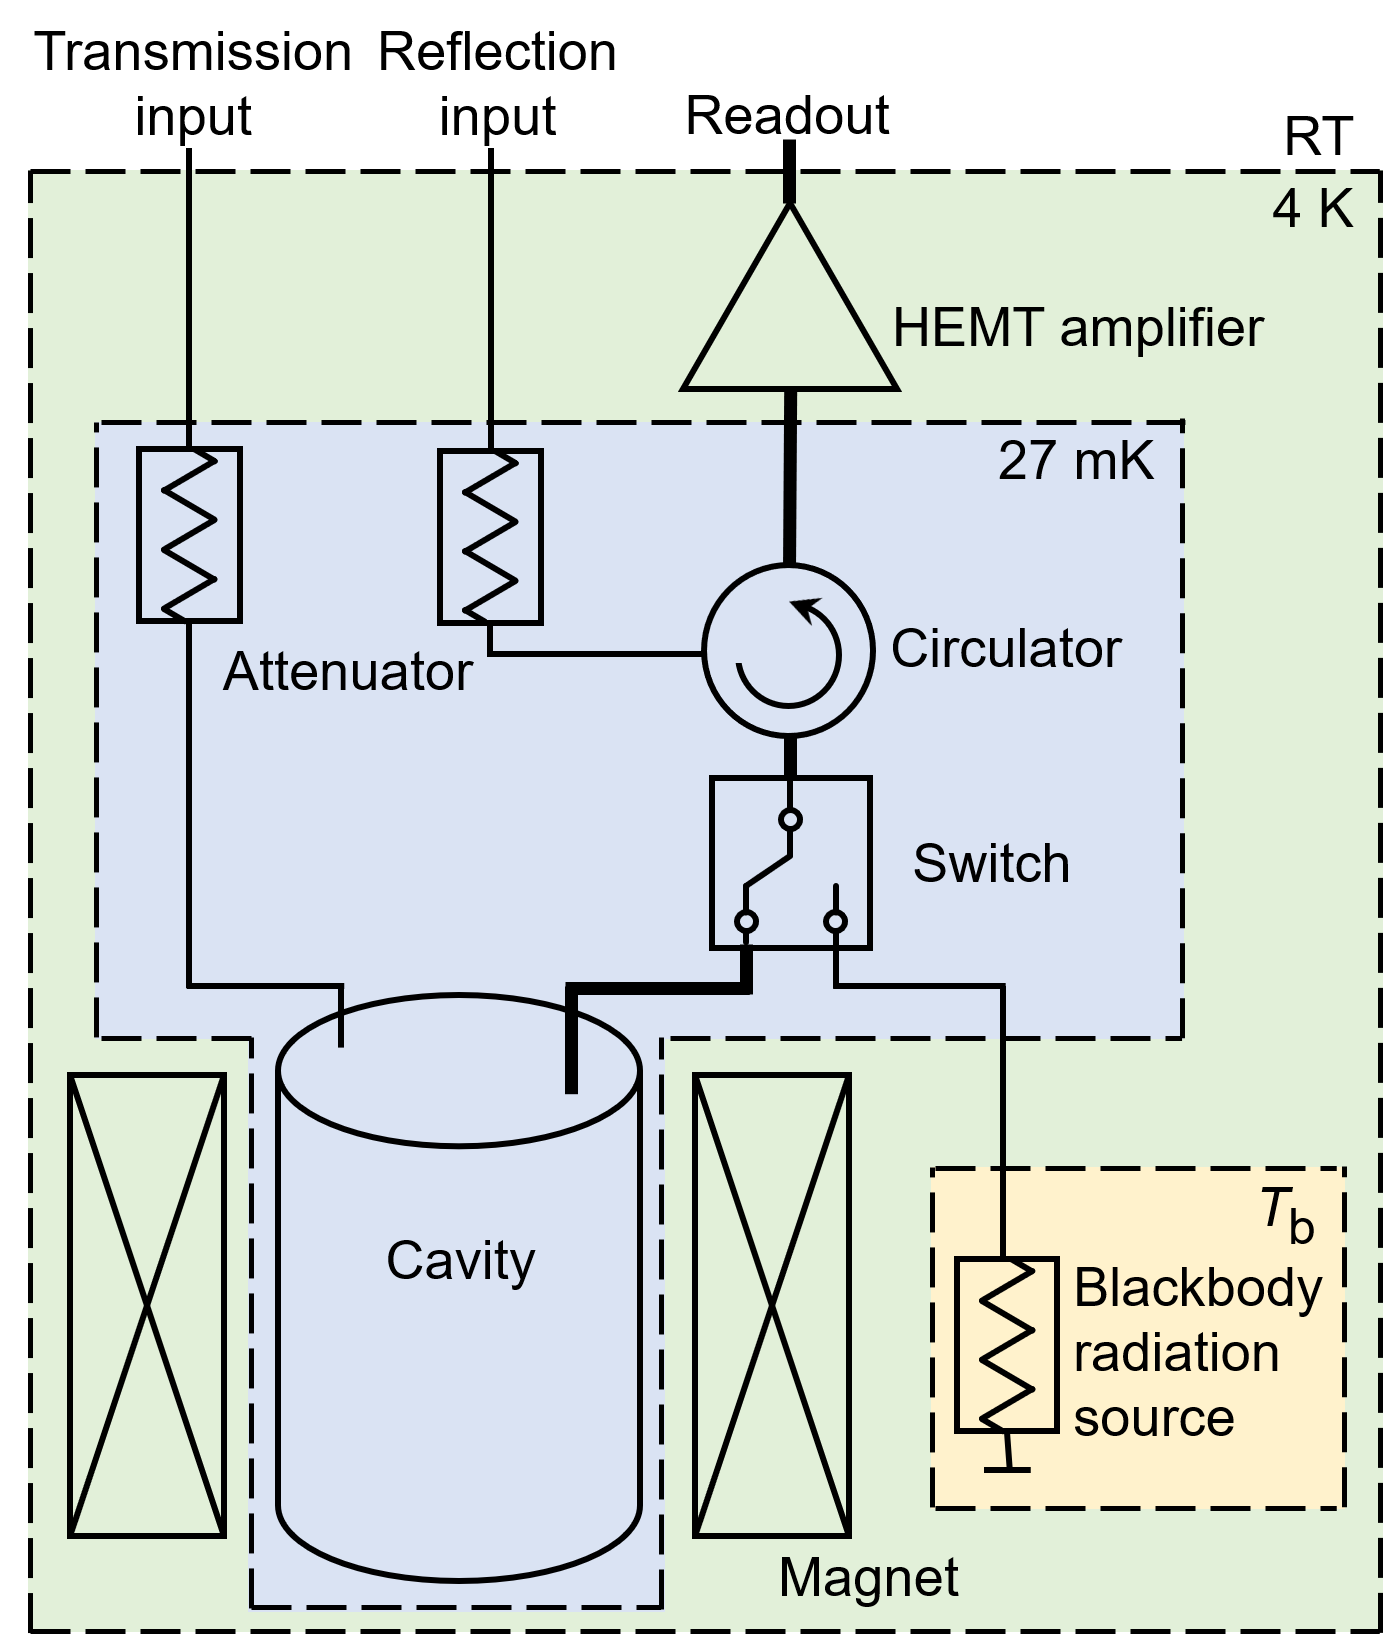
\includegraphics[width=8.6cm]{figures/colored_Simplified_wiring_V3.png}
  \caption{%
The simplified diagram of the TASEH apparatus.}
  \label{fig:TASEH}
\end{figure}


The signal power extracted from a MW cavity on resonance is given 
by~\cite{AxionFormula,HAYSTACIII}:
\begin{equation}
%P_s = \left(\bggamma^2\frac{\alpha^2\hbar^3c^3\rho_a}{\pi^2\Lambda^4}\right)\times
%\left(\omega_c\frac{1}{\mu_0}B_0^2VCQ_L\frac{\beta}{1+\beta}\right).
P_s = \left(\bgagg^2\frac{\hbar^3c^3\rho_a}{m_a^2}\right)\times
\left(\omega_c\frac{1}{\mu_0}B_0^2VCQ_L\frac{\beta}{1+\beta}\right).
\label{eq:ps}
\end{equation}
The first set of parentheses contains \bgagg, $m_a$, physical constants, 
and the local dark-matter density 
$\rho_a=0.45~\GeV/\mathrm{cm}^3$~\cite{[{}][{. Both $0.45~\GeV/\mathrm{cm}^3$ 
(used by ADMX, HAYSTAC, CAPP, and QUAX-$a\gamma$) and $0.3~\GeV/\mathrm{cm}^3$ 
(more commonly cited by the other direct DM search experiments) are consistent 
with the recent measurements.}]Read:2014qva,PDG}. 
For the QCD axions, the \bgagg\ 
is related to the axion mass \ma: 
\begin{equation}
 \bgagg = \left(\frac{\bggamma\alpha}{\pi \Lambda^2}\right)\ma, 
\label{eq:grelation}
\end{equation}
where $\bggamma$ is a dimensionless model-dependent parameter,    
with numerical values -0.97 and 0.36 
in the Kim-Shifman-Vainshtein-Zakharov (KSVZ)~\cite{KSVZI,KSVZII} and 
the Dine-Fischler-Srednicki-Zhitnitsky (DFSZ)~\cite{DFSZI,DFSZII} benchmark 
models, respectively. The $\alpha$ is the 
fine-structure constant and  $\Lambda=78~\MeV$ is a scale parameter that can 
be derived from the mass and the decay constant of the pion and the ratio of 
the up to down quark masses. 
%
The second set of parentheses contains parameters related to the experimental 
setup: 
%The parameters related to the experimental setup include: 
the angular resonant frequency of the cavity $\omega_c$, the vacuum 
permeability $\mu_0$, the nominal strength of the external magnetic field 
$B_0$, the effective volume of the cavity $V$, and the loaded quality factor 
of the cavity \(Q_L=Q_0/(1+\beta)\), where $Q_0$ is the unloaded, intrinsic 
quality factor and $\beta$ is the coupling coefficient which 
determines the amount 
of coupling of the signal to the receiver. The form factor $C$ is the 
normalized overlap of the electric field 
$\vec{\bm{E}}$, for a particular cavity resonant mode, with the external 
magnetic field $\vec{\bm{B}}$:
\begin{equation}
  C = \frac{\left[\int\left( \vec{\bm{B}}\cdot\vec{\bm{E}}\right) d^3\bm{x}\right]^2}{B_0^2V\int E^2 d^3\bm{x}}.
\label{eq:formfactor} 
\end{equation} 
The magnetic field $\vec{\bm{B}}$ in TASEH points mostly along the axial
direction of the cavity. 
For cylindrical cavities, the largest form factor is from the 
TM$_{010}$ mode. The expected signal power derived from the experimental 
parameters of TASEH is $P_s\simeq 1.4\times10^{-24}$~W for a KSVZ axion 
with a mass of 19.6\muevcc. 

In the haloscope experiments, the figure of merit that determines the design 
of the experimental setup is the signal-to-noise ratio
(SNR), i.e. the ratio of the signal power $P_s$ to the fluctuation in 
the averaged noise power spectrum $\sigma_n$~\cite{Dicke}, given by:  
%According to Dicke's Radiometer Equation~\cite{Dicke}, the $\sigma_n$ 
%is given by: 
%\begin{equation}
% \sigma_n  =  k_B\tsys\sqrt{\frac{\Delta f}{t}}, 
% \label{eq:sigman}
%\end{equation}
%where \tsys\ is the system noise temperature, an effective 
%temperature associated with the total noise of the system, 
%$t$ is the data integration time and $\Delta f$ is the resolution bandwidth. 
%Assuming that all the axion signal power falls within $\Delta f$, 
%the SNR will therefore be:
\begin{equation}
   \text{SNR}  =  \frac{P_s}{\sigma_n}=  \frac{P_s}{k_B\tsys}\sqrt{\frac{t}{\Delta f}},
 \label{eq:SNR}
\end{equation}  
where \tsys\ is the system noise temperature, an effective 
temperature associated with the total noise of the system, 
$t$ is the data integration time, and $\Delta f$ is the resolution bandwidth. 
Here, one assumes that all the axion signal power falls within $\Delta f$.  


The system noise temperature \tsys\ has three major components:
\begin{equation}
 \tsys = \Tilde{T}_\text{mx} + \left(\Tilde{T}_\text{c}-\Tilde{T}_\text{mx}\right)L(\omega) + \ta,
\label{eq:pn}
\end{equation}
where $\omega$ is the angular frequency.
The last term \ta\ is the effective temperature of the
noise added by the receiver (mainly from the first-stage amplifier).
The sum of the first two terms is equivalent 
to the sum of the reflection of the incoming noise from
the attenuator anchored to the mixing flange (Fig.~\ref{fig:TASEH}) 
and the transmission of the noise from the cavity body itself.
The
$\Tilde{T}_i=\left(\frac{1}{e^{\left.\hbar\omega\middle/k_BT_i\right.}-1} + \frac{1}{2}\right)\left. \hbar\omega\middle/k_B\right.$ refers to
the effective temperature due to
the blackbody radiation at a physical temperature $T_i$ and
the vacuum fluctuation.
%The $T_\text{c}\simeq155$~mK and $T_\text{mx}\simeq27$~mK are the physical
%temperatures of the cavity and of the mixing flange, respectively. 
The difference
of the effective temperatures $\Tilde{T}_\text{c}-\Tilde{T}_\text{mx}$ is
modulated by a Lorentzian function $L(\omega)$. 
If the physical temperatures of the cavity $T_\text{c}$ and of 
the mixing flange $T_\text{mx}$ 
are identical, the thermal noise spectrum from the cavity is flat. 
The derivation of the first two terms in Eq.~\eqref{eq:pn} can be found in
Ref.~\cite{TASEHAnalysis}. 

%Therefore, 
%Via the
%cryogenic switch, the noise from the blackbody radiation source with a 
%controlled temperature $T_{\text b}$ is used to calibrate the added noise and 
%the overall gain of the amplification chain. 
The calibration for the amplification chain is performed by 
connecting the HEMT to a blackbody radiation source (Fig.~\ref{fig:TASEH}) 
instead of the cavity via a cryogenic switch.  
Various values of input currents are sent to the 
source to change its temperature $T_{\text b}$ monitored by a thermometer. 
The output power is fitted to a first-order polynomial, as a function of
the source temperature, to extract the overall gain and added noise \ta. 


The data for the analysis presented here were collected by TASEH 
from October 13, 2021 to November 15, 2021, and are termed as the CD102 data, 
where CD stands for ``cool down''. 
The CD102 data cover the frequency range of \flo--\fhi~GHz. In this Letter, 
most of the frequencies in unit of GHz are quoted with five decimal places as 
the absolute accuracy of frequency is $\approx 10$~kHz. It shall be noted 
that the frequency resolution is 1~kHz.  
During the CD102 data run, 
the temperature of the cavity stayed at $T_\text{c}\simeq155$~mK, higher 
with respect to the mixing flange $T_\text{mx}\simeq27$~mK; it is believed 
that the cavity had an 
unexpected thermal contact with the radiation shield in the DR. 
As a result, the $\Tilde{T}_\text{c}$ and $\Tilde{T}_\text{mx}$ 
are 0.18~K and 0.11~K, respectively. 
The form factor $C$ for 
the TM$_{010}$ mode varies from 0.60 to 0.61 over the operational 
frequency range. 
The $Q_0$ at the cryogenic temperature is $\simeq 60700$. 
The insertion depth of the readout probe is set for 
$\beta\simeq2$ since this value, for a given amount 
of time and a fixed value of SNR, maximizes the frequency coverage. 
In this case, 
the cavity line width, $\left.\omega_c\middle/2\pi Q_L\right.$, is about 
240~kHz. 

The calibration was carried out before, during, and after the data taking,
which showed that the performance of the system was stable over time. 
The \ta\ obtained from the calibration is 
about \noise~K, with a frequency dependence. In CD102, 
there were 837 resonant-frequency steps in total, with a frequency difference 
of $\Delta f_\text{s}=95-115$~kHz between the steps. The value of 
$\Delta f_\text{s}$ was kept within 10\% of 105~kHz ($\lesssim$ half of the 
cavity line width) rather than 
a fixed value, such that the rotation angle of the tuning rod did not need to 
be fine-tuned and the operation time could be minimized. A 10\% variation of 
the $\Delta f_\text{s}$ is found to have no impact on the \bgagg\ limits. 
Each resonant-frequency step is denoted as a ``scan'' 
and the data integration time was about 32-42 minutes. 
The variation of the integration time was introduced to compensate 
the frequency dependence of the added noise. 

%



%%% analysis and results

   The analysis of the CD102 data follows the procedure similar to that 
developed by the HAYSTAC experiment~\cite{HAYSTACII} and the details are 
described in Ref.~\cite{TASEHAnalysis}. The fast Fourier transform 
algorithm is performed on the IQ time series data to obtain the 
frequency-domain power spectrum. 
The Savitzky-Golay (SG) 
filter~\cite{SGFilter} is applied to model the Lorentzian structure of 
the background caused by the temperature difference between the cavity and 
the mixing flange [Eq.~\eqref{eq:pn}] and to obtain the 
the average noise power. 
Deviations from the average noise power are compared with the 
uncertainty on the averaged power spectrum, which defines the 
observed SNR. All the spectra from different 
frequency scans, particularly for the frequency bins that appear in 
multiple spectra, are combined with a weighting algorithm. 
%The uncertainty of the averaged power at the overlapped region is
%reduced due to the combination. 
In order to maximize the SNR, a running window of 
five consecutive bins in the combined spectrum is applied and the five bins 
within each window are merged to construct a final spectrum. 
The five frequency bins correspond to the 5-kHz axion signal line width,  
assuming a standard Maxwellian axion line shape with a velocity 
variance $\left<v^2\right>=$(270~km/s)$^2$~\cite{HAYSTACII}. 
%as described 
%by Eq.~\eqref{eq:simplesignal}. 
This line shape is also used when defining the maximum likelihood 
weights for merging. 
%\begin{equation}
%\mathcal{F}(f, f_a) = \frac{2}{\sqrt{\pi}}\sqrt{f-f_a}\left(\frac{3}{\alpha}\right)^{3/2}
%e^{\frac{-3\left(f-f_a\right)}{\alpha}},
%\label{eq:simplesignal}
%\end{equation}
%where $\alpha\equiv  f_a \left<v^2\right>/c^2$. 
%Here, the frequency $f$ must be greater or equal to the axion frequency 
%$f_a=\left.\ma c^2\middle/h\right.$. 
%In this standard assumption, 
%the DM halo density distribution is assumed 
%to be spherically symmetric and close to be isothermal, which results in a 
%velocity distribution similar to the Maxwell-Boltzmann distribution. 
%Therefore, the variance $\left<v^2\right>$ and the most probable velocity 
%$v_p$ are related to each other:
%$\left<v^2\right>=3v_p^2/2=$(270~km/s)$^2$, where $v_p=220$~km/s is the local
%circular velocity of DM in the galactic rest frame and this value is also
%used by other axion experiments.


After the merging, 22 candidates with an SNR greater than 3.355 were found and 
a rescan was performed to check if they were real signals  
or statistical fluctuations.        
Among them, 20 candidates were from the fluctuations because they were gone 
after a few rescans. 
The remaining two candidates, in the frequency ranges of 
4.71017 -- 4.71019~GHz and 4.74730 -- 4.74738~GHz, are not 
considered axion signal candidates for the following reasons. 
The signal in the second frequency range was detected via a portable antenna 
outside the DR and found 
to come from the instrument control computer in the laboratory, while the 
signal in the first frequency range was not 
detected outside the DR but still present after 
turning off the external magnetic field. 
No limits are placed for the above two frequency ranges.  

%% results
Since no candidates were found after the rescan, the upper limits 
at 95\% confidence level (C.L.) on the \gagg\ are derived by setting the 
maximum SNR equal to five, 
with the assumption that axions make up 100\% of the local dark matter 
density.  
Figure~\ref{fig:gaggall} shows the \gagg\ limits of TASEH and the 
ratios relative to the KSVZ benchmark value,  
 together with those from the previous searches. 
The limits on 
\gagg\ range from \lolimit\GeVinv\ to \hilimit\GeVinv, with an average 
value of \avelimit\GeVinv; the lowest value comes from the frequency bins with 
additional eight times more data from the rescans, while the highest value 
comes from the frequency bins near the boundaries of the spectrum. 
Overall the total relative systematic uncertainty is 
$\approx 4.6\%$, coming from the uncertainties on the loaded quality 
factor $Q_L$, the coupling coefficient $\beta$, the added noise temperature 
\ta, the effect of the misalignment between the true axion frequency and 
the lower boundaries of the frequency bins, and the variation of the 
SG-filter parameters. 


The analysis that merges bins without 
assuming a signal line shape results in $\approx5.5$\% larger values on the 
\gagg\ limits. If a Gaussian signal line shape with an FWHM of 2.5~kHz  
 is assumed instead, the limits will be $\approx3.8$\% smaller than the 
central results. If the \gagg\ limits are derived from the observed SNR as 
described in the ADMX paper~\cite{ADMXVIII}, 
rather than using the 5$\sigma$ target SNR, the average limit on \gagg\ will 
be $\approx\ADMXavelimit\GeVinv$. 




\begin{figure*} 
  \centering
  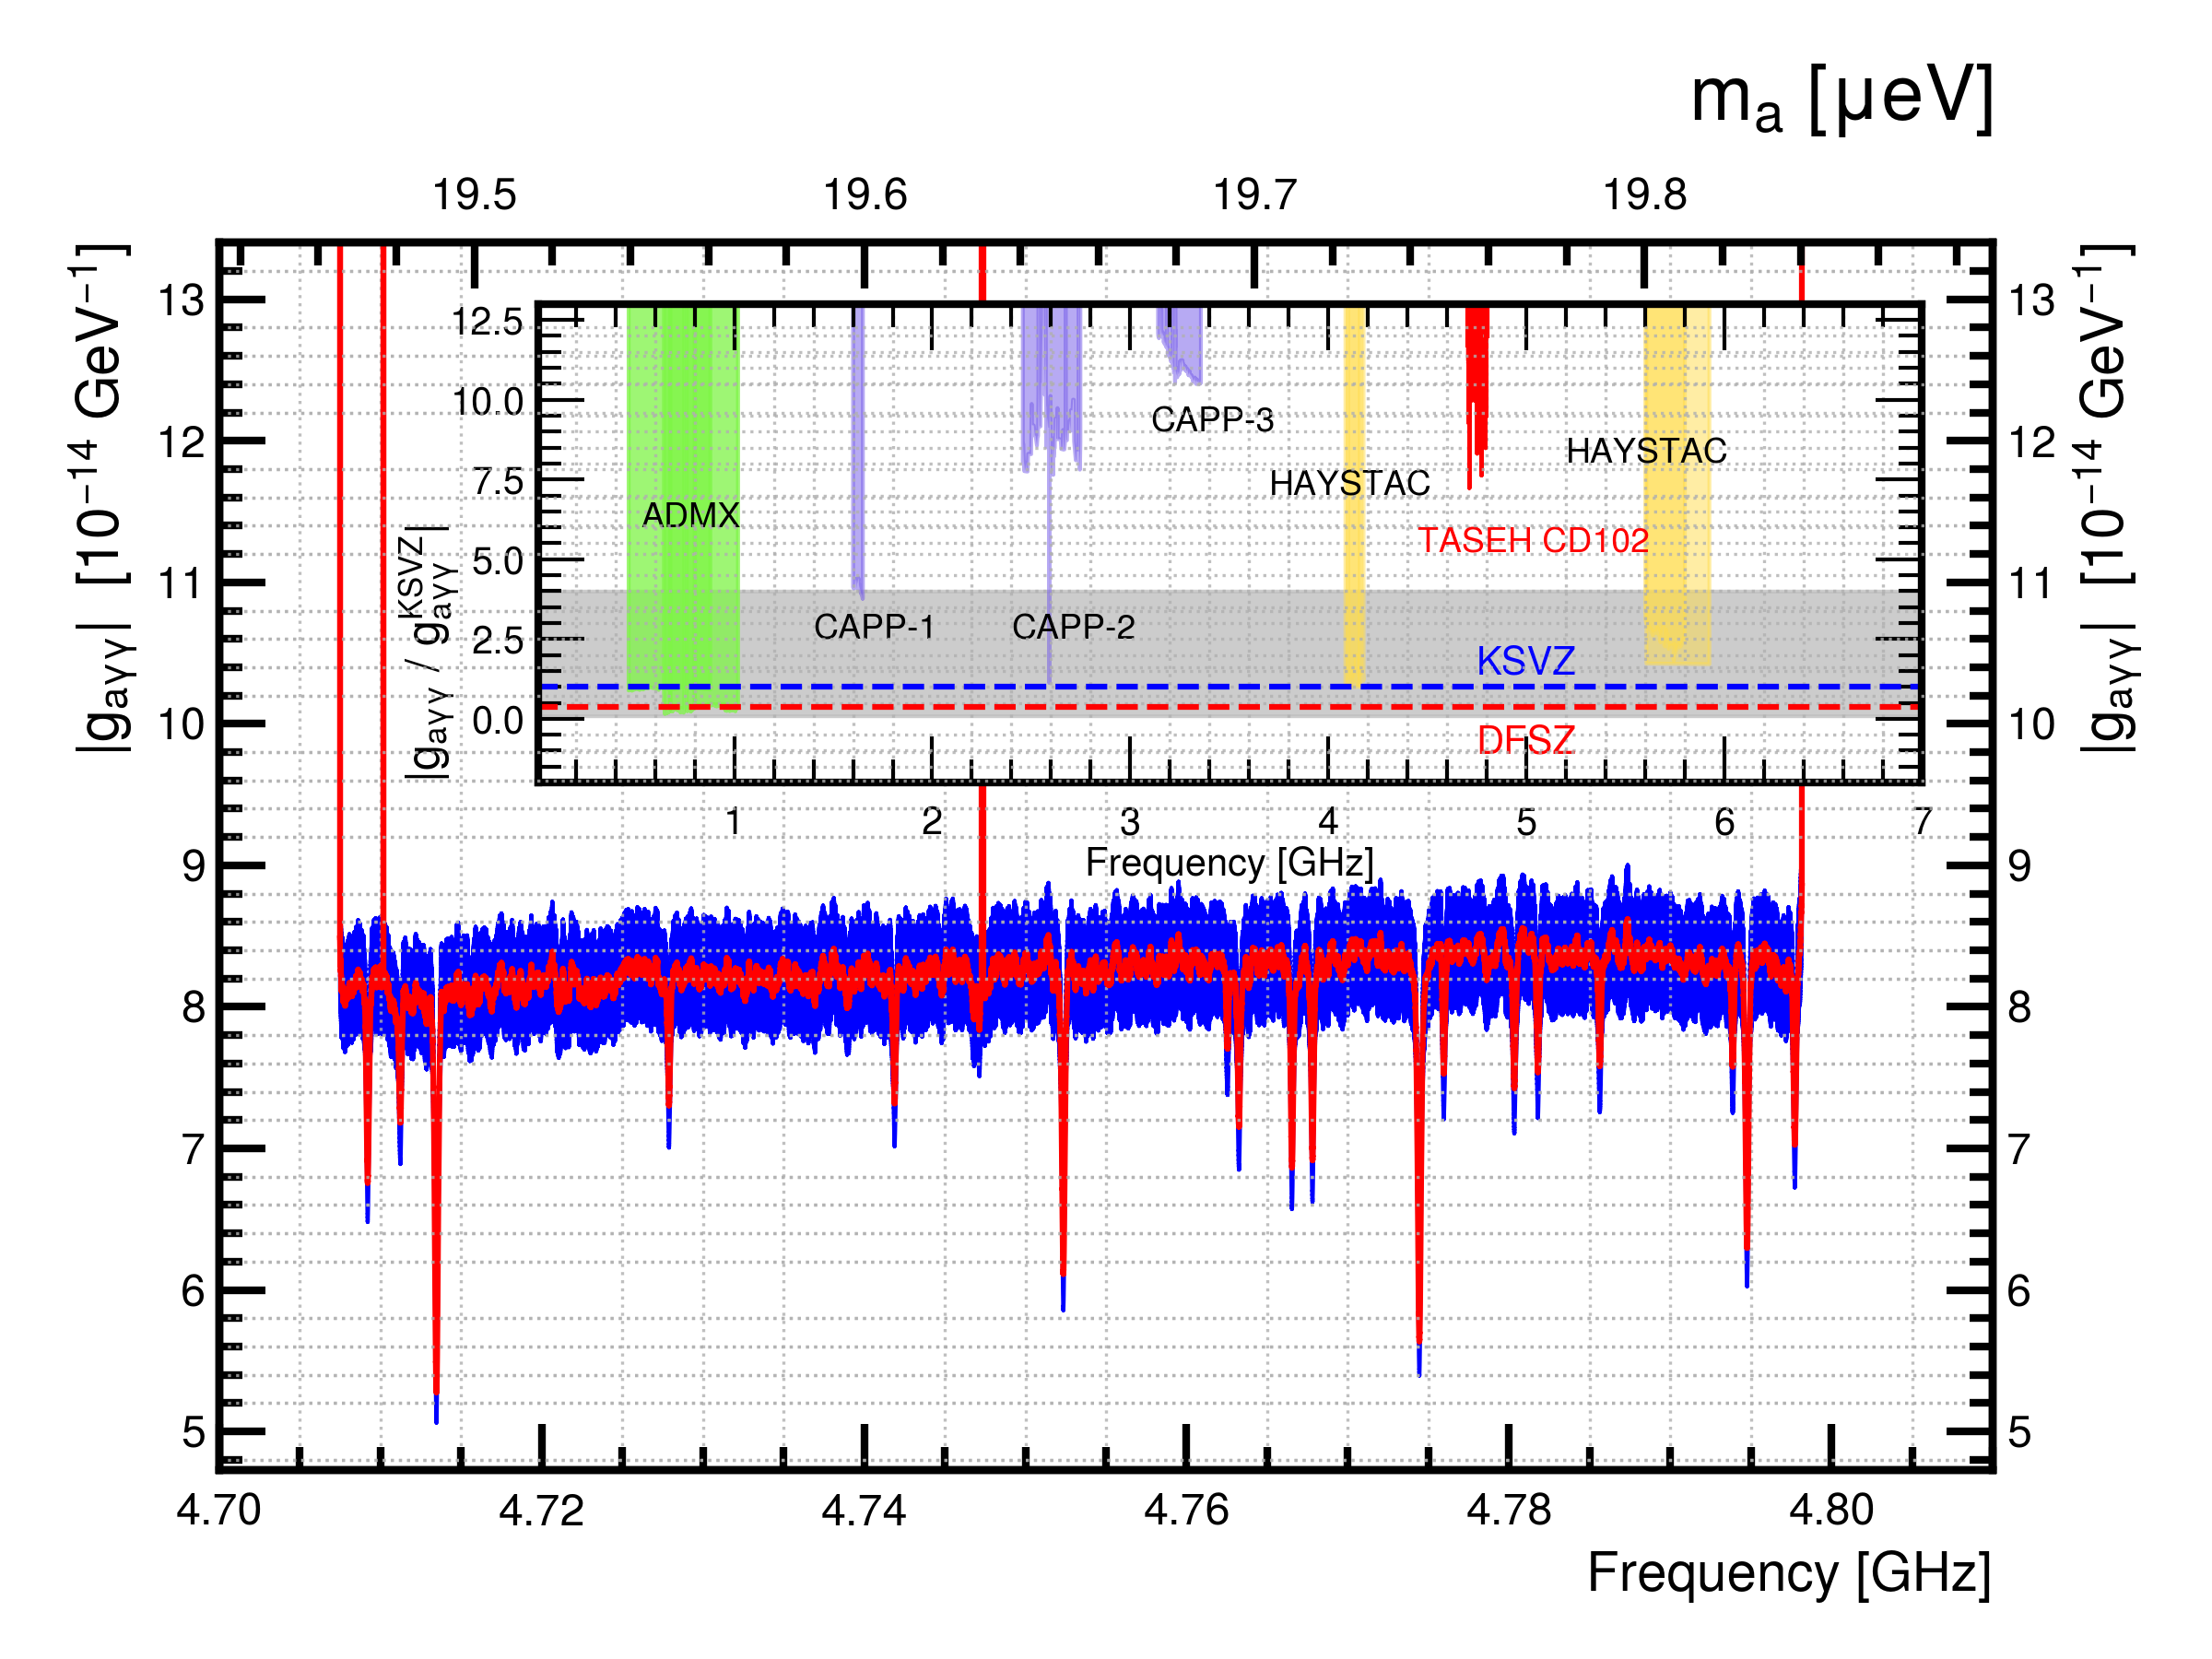
\includegraphics[width=12.9cm]{figures/combineTASEH_all.png}
%  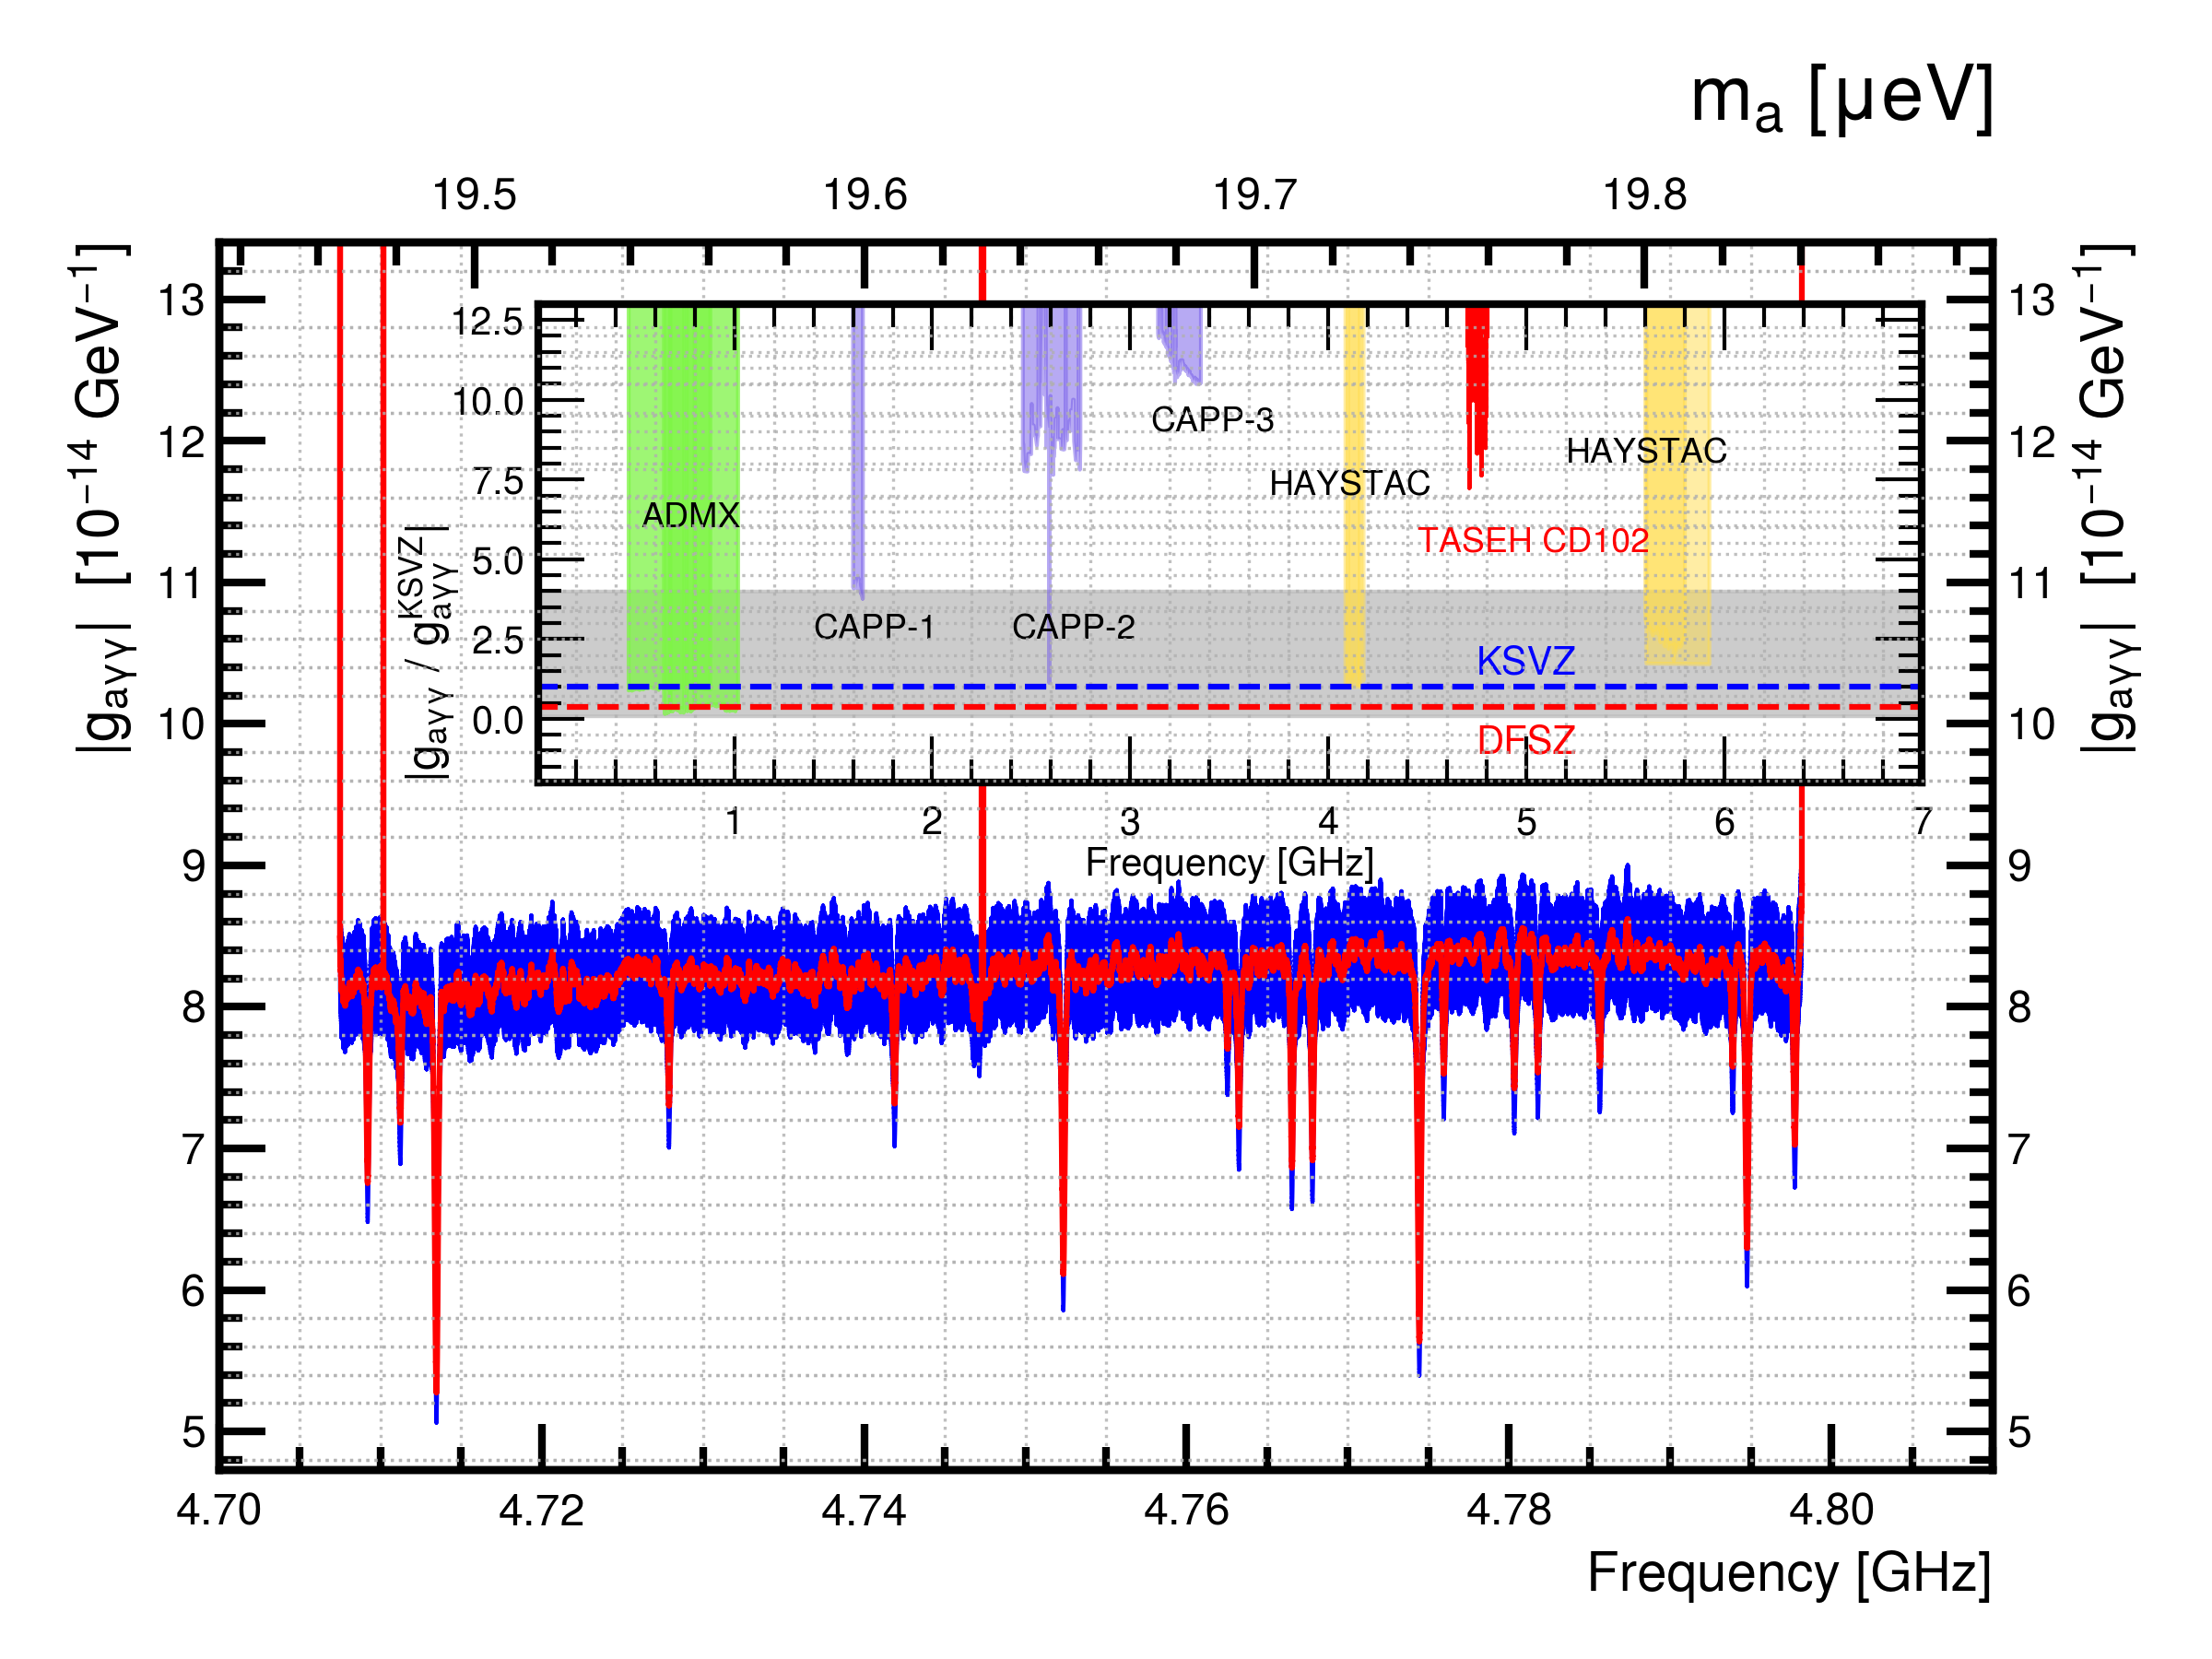
\includegraphics[width=17.2cm]{figures/combineTASEH_all.png}
  \caption{The 95\% C.L. limits on \gagg\ from TASEH and the ratio of the 
limits with respect to the KSVZ benchmark value 
 from the CD102 data (red band) and previous searches performed by the 
 ADMX, CAPP, and HAYSTAC Collaborations (inset). 
 The blue error band indicates the systematic 
  uncertainties. The gray band in the inset shows the allowed region of 
 \gagg\ vs. $m_a$ 
 from various QCD axion models, while the blue and red dashed lines are the 
values predicted by the KSVZ and DFSZ benchmark models, respectively.
 }

  \label{fig:gaggall}
\end{figure*}




%%%% faxion
After the collection of the CD102 data, 
synthetic axion signals were injected into the cavity and read out via the 
same transmission line and amplification chain. 
%Due to the uncertainties on the losses of signal transmission
% lines, the synthetic axion signals are not used to perform an absolute 
%calibration of the search sensitivity. Instead, 
%a test with synthetic axion signals could be used to verify the procedures of 
%data acquisition and physics analysis. 
The procedure to generate axion-like signals is summarized in 
Ref.~\cite{TASEHInstrumentation} and the analysis of the synthetic axion 
data is described in Ref.~\cite{TASEHAnalysis}. 
The analysis results demonstrates
the capability of the experimental setup and the analysis strategy to discover
an axion signal with 
$\gagg\approx {\cal O}\left(10\left|\bgagg^\text{KSVZ}\right|\right)$.


%% conclusion 
In summary, a search for axions in the mass 
range $\mlo < \ma < \mhi \muevcc$ was performed by the TASEH Collaboration.  
Apart from the non-axion signals, no candidates with a significance more than
3.355 were found. The experiment excludes models with the 
axion-two-photon coupling $\gagg\gtrsim \avelimit\GeVinv$ at 95\% C.L.,
 a factor of eleven 
above the benchmark KSVZ model. The sensitivity on \gagg\ reached by TASEH 
is three orders of magnitude better than the existing limits in the same 
mass range.  
It is also the first time that a haloscope-type experiment places 
constraints in this mass region. 
The target of TASEH is to search for axions in the mass range of 
16.5--20.7\muevcc\ corresponding to a frequency range of 4--5~GHz. 
%In the coming years, several upgrades are expected, including: the use of a 
%quantum-limited Josephson parametric amplifier as the first-stage amplifier, 
%the replacement of the existing dilution refrigerator with a new one that has 
%a magnetic field of about 9~Tesla and a larger bore size, and the development 
%of a new cavity with a significantly larger effective volume. 
With the upcoming upgrades of the experimental setup and several years of data 
taking, TASEH is expected to probe the QCD axion band in the target mass range.

\begin{acknowledgments}
We thank Chao-Lin Kuo for his help to initiate this project as well as
discussions on the microwave cavity design, Gray Rybka and Nicole Crisosto
for their introduction of the ADMX experimental
setup and analysis, Anson Hook for the discussions and the review of the
axion theory, and Jiunn-Wei Chen, Cheng-Wei Chiang, Cheng-Pang Liu, and
Asuka Ito for the discussions of future improvements in axion searches. 
We acknowledge support of microwave test and measurement equipment from the 
National Chung-Shan Institute of Science and Technology. 
  The work of the TASEH Collaboration was funded by
the Ministry of Science and Technology (MoST) of Taiwan with grant numbers
MoST-109-2123-M-001-002, MoST-110-2123-M-001-006, MoST-110-2112-M-213-018,
MoST-110-2628-M-008-003-MY3,
and MoST-109-2112-M-008-013-MY3, and by the Institute of Physics, Academia
Sinica.
\end{acknowledgments}
\bibliographystyle{apsrev4-2}
\bibliography{letter}% Produces the bibliography via BibTeX.

\end{document}
%
% ****** End of file apssamp.tex ******
